\chapter{\label{cha:uniform-results-discussion} Uniform Grids -- Results and Discussion}

\section{Results}

\subsection{Navier-Stokes}




\begin{figure}
    \centering
    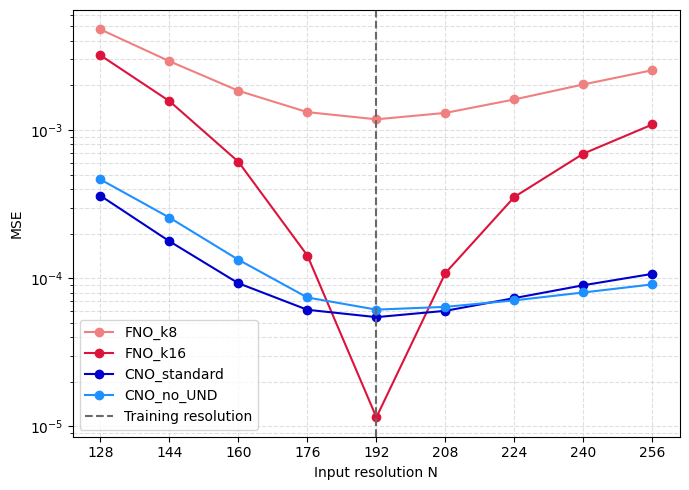
\includegraphics[width=0.8\textwidth]{figures/loss_vs_resolution_navier_stokes.png}
    \caption{\label{fig:loss_vs_resolution_navier_stokes} A plot of the MSE loss as a function of resolution for the four models trained on the Navier-Stokes dataset. The training resolution is indicated by the vertical dashed line.}
\end{figure}

\begin{table}
    \centering
    \caption{\label{tab:d-values-navier-stokes} Discretization variance value $D$ for the Navier-Stokes uniform-grid experiment. Lower values indicate that the loss remains more consistent across evaluation resolutions relative to the loss at the training resolution.}
    \begin{tabular}{lc}
        \hline
        Model & $D$ \\
        \hline
        FNO\_k8 & 0.5076 \\
        FNO\_k16 & 3.4817 \\
        CNO\_standard & 0.5854 \\
        CNO\_no\_UND & 0.5847 \\
        \hline
    \end{tabular}
\end{table}

The four models outlined in Section~\ref{uniform-experiments} were
evaluated on the Navier-Stokes dataset. Figure~\ref{fig:loss_vs_resolution_navier_stokes}
shows the mean squared error (MSE) loss as a function of evaluation resolution for each
model, with the training resolution indicated by the vertical dashed
line. Table~\ref{tab:d-values-navier-stokes} reports the discretization
variance value $D$, which measures how much the loss changes across
resolutions relative to the loss at the training resolution.

Among the FNO models, FNO\_k16 achieves the lowest loss at the training
resolution, but also has the largest value of $D$. Its performance
therefore changes the most under resolution transfer. This contrast is
especially pronounced at the lowest tested resolution, where the loss of
FNO\_k16 increases by more than two orders of magnitude compared with
its loss at the training resolution. FNO\_k8 has a higher loss at all tested resolutions including the training resolution, but a substantially lower value of $D$, indicating
a more consistent loss across the evaluated resolutions. For both FNO
variants, the loss increases more rapidly when evaluating below the
training resolution than when evaluating above it.

The two CNO variants show much flatter loss curves than FNO\_k16 and
have nearly identical values of $D$. Their training-resolution losses are
also comparable. The standard CNO performs slightly better at the
training resolution, at lower resolutions, and at $N = 208$. At the
highest evaluated resolutions, CNO\_no\_UND gives slightly lower losses
than CNO\_standard. Overall, the Navier-Stokes results show a trade-off:
FNO\_k16 gives the best performance at the training resolution, while
FNO\_k8 and the CNO variants show more consistent behavior across
resolutions.



\subsection{Darcy flow}

\begin{figure}
    \centering
    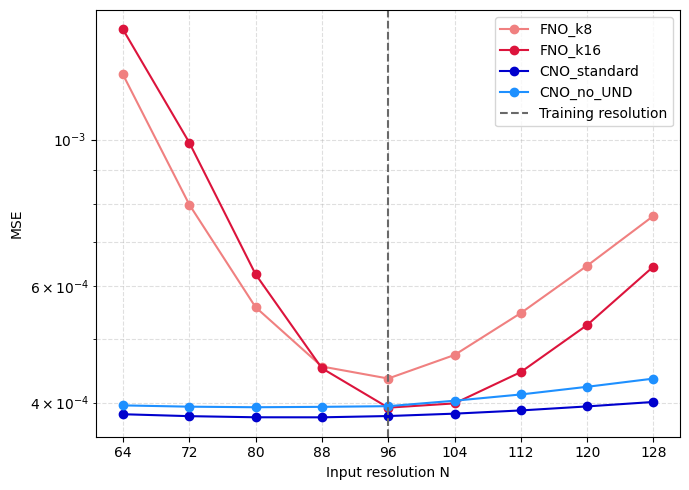
\includegraphics[width=0.8\textwidth]{figures/loss_vs_resolution_darcy_flow.png}
    \caption{\label{fig:loss_vs_resolution_darcy_flow} A plot of the MSE loss as a function of resolution for the four models trained on the Darcy flow dataset. The training resolution is indicated by the vertical dashed line.}
\end{figure}


To test whether the trends observed on the Navier-Stokes dataset also
appear on a qualitatively different PDE benchmark, the four models were
evaluated on the Darcy flow dataset. The Darcy flow dataset was chosen as the solution space is smooth, making it a good point of comparison to the Navier-Stokes dataset. Figure~\ref{fig:loss_vs_resolution_darcy_flow}
shows the MSE loss as a function of evaluation resolution for each
model, with the training resolution indicated by the vertical dashed
line. Table~\ref{tab:d-values-darcy-flow} reports the corresponding
discretization variance value $D$.

\begin{table}
    \centering
    \caption{\label{tab:d-values-darcy-flow} Discretization variance value $D$ for the Darcy flow uniform-grid experiment. Lower values indicate that the loss remains more consistent across evaluation resolutions relative to the loss at the training resolution.}
    \begin{tabular}{lc}
        \hline
        Model & $D$ \\
        \hline
        FNO\_k8 & 0.3583 \\
        FNO\_k16 & 0.4179 \\
        CNO\_standard & 0.0140 \\
        CNO\_no\_UND & 0.0260 \\
        \hline
    \end{tabular}
\end{table}

Compared with the Navier-Stokes experiment, the four models are closer
in overall performance on the Darcy flow dataset. At the training
resolution, CNO\_standard achieves the lowest loss, followed by
FNO\_k16, CNO\_no\_UND, and FNO\_k8. The two FNO variants show a similar
pattern to that observed for Navier-Stokes; the loss is lowest near the
training resolution and increases when the model is evaluated at other
resolutions. This increase is stronger below the training resolution
than above it. Notably, FNO\_k8 outperforms FNO\_k16 at resolutions below $N = 88$. This indicates that
retaining more Fourier modes does not consistently improve performance
under transfer to coarser grids.

The CNO variants show much flatter loss curves across the evaluated
resolutions, with $D$ values of order \(10^{-2}\). At lower resolutions,
both CNO models maintain an almost constant loss, while at higher
resolutions both losses increase slowly. In contrast to the
Navier-Stokes experiment, CNO\_standard outperforms CNO\_no\_UND at all
evaluated resolutions. The loss of CNO\_no\_UND also increases more
quickly than that of CNO\_standard when evaluating above the training
resolution. Overall, the Darcy flow results show a clearer separation
between the FNO and CNO variants in terms of discretization robustness;
the FNO models are more sensitive to resolution transfer, while the CNO
models remain nearly constant across the tested range.


\subsubsection{FNO resolution-transfer diagnostics}\label{sec:fno_diagnostics}

The results in Figures~\ref{fig:loss_vs_resolution_navier_stokes} and~\ref{fig:loss_vs_resolution_darcy_flow} show that the FNO variants are more sensitive to changes in evaluation resolution than the CNO variants. This effect is most pronounced for FNO\_k16 on the Navier--Stokes dataset, which achieves a low loss at the training resolution but a substantially higher loss away from it. To investigate this behavior in more detail, three additional diagnostics were performed using FNO\_k16 on the Navier--Stokes dataset. These diagnostics were evaluated at the lowest tested resolution \(N=128\), the training resolution \(N=192\), and the highest tested resolution \(N=256\).

\begin{figure}
    \centering
    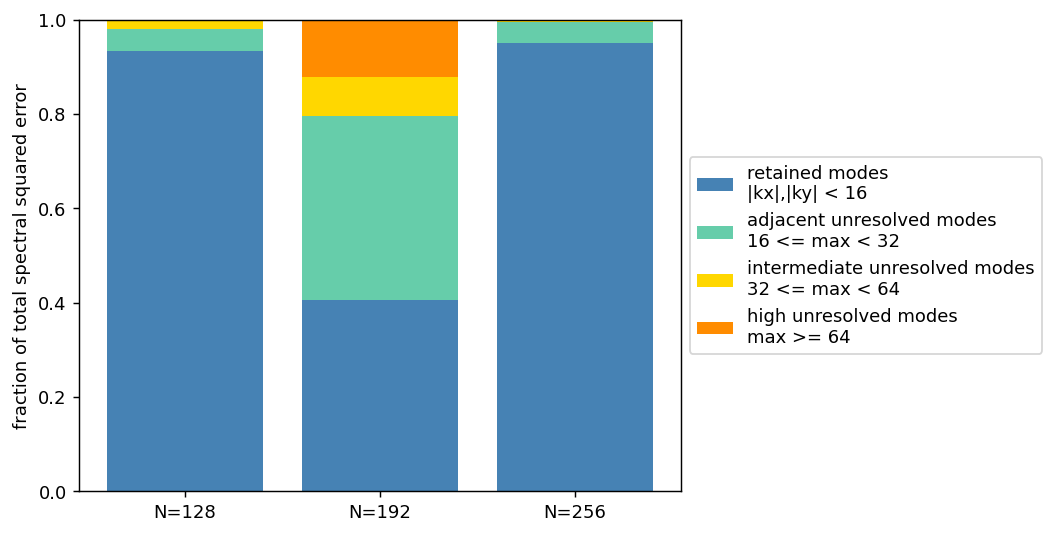
\includegraphics[width=0.85\textwidth]{figures/fno_error_bands.png}
    \caption{Fraction of total spectral squared error by Fourier box band for FNO k16 on the Navier--Stokes dataset. Here max denotes \(max(|k_x|,|k_y|)\). The first band, \(|k_x|,|k_y|<16\), corresponds to the modes retained by the FNO\_k16 spectral convolution.}
    \label{fig:fno_error_bands}
\end{figure}

First, the prediction error was decomposed in Fourier space. For each of the three resolutions, the pointwise difference between the model prediction and the ground truth was computed and transformed into Fourier space. The squared magnitudes of the resulting Fourier coefficients were then grouped into bands. The first band, \(|k_x|,|k_y|<16\), corresponds to the Fourier modes retained by the FNO k16 model. Figure~\ref{fig:fno_error_bands} shows the fraction of total spectral squared error in each band for \(N=128\), \(N=192\), and \(N=256\).

At the training resolution \(N=192\), the error is distributed across several spectral bands. The retained modes account for approximately \(40.6\%\) of the total spectral error, while the adjacent unresolved modes account for approximately \(39.1\%\). At the transfer resolutions, the distribution changes substantially: the retained modes account for approximately \(93.3\%\) of the error at \(N=128\) and \(95.1\%\) at \(N=256\). Since the overall prediction error is much larger at these transfer resolutions, this indicates that the increased error is concentrated primarily in the modes explicitly retained by the FNO, rather than only in modes outside the spectral cutoff.

This diagnostic localizes the error, but does not by itself identify its cause. The following diagnostics therefore test whether this retained-mode error comes from changes in the represented input and target spectra, or from changes introduced during the FNO forward pass.

Second, a spectral-resampling control experiment was performed to separate changes in represented spectral content from changes in spatial evaluation resolution. In the original resolution transfer experiment, fields at different resolutions were obtained using bicubic interpolation. This can slightly change the retained Fourier coefficients of the input and target fields, which makes it difficult to determine whether the observed prediction drift is caused by changes in the represented data or by evaluating the FNO on a different grid.

To test this, the experiment was repeated using spectral resampling. Starting from the \(N=192\) input and target fields, new \(N=128\) and \(N=256\) versions were constructed directly in Fourier space. This produces different grid representations of the same spectrally defined fields. The FNO was then evaluated on both the bicubic-resampled and spectrally resampled fields.

To quantify how much the retained spectral content changes, the retained Fourier coefficients of the input, target, and prediction were compared to their corresponding \(N=192\) coefficients. Because fields at different spatial resolutions have different numbers of grid points, they cannot be compared directly pointwise. The retained Fourier coefficients provide a common representation for the modes shared across resolutions. The following drift measure is therefore used only as a diagnostic for comparing these shared retained modes, not as a general prediction-error metric. For a field \(v\), this drift is defined as
\begin{equation}
\delta_{\mathrm{ret}}(v;N)
=
\frac{
\left\|\hat v_{\mathrm{ret}}^{N}-\hat v_{\mathrm{ret}}^{192}\right\|_2
}{
\left\|\hat v_{\mathrm{ret}}^{192}\right\|_2
},
\label{eq:retained-mode-drift}
\end{equation}
where \(\hat v_{\mathrm{ret}}^{N}\) denotes the vector of retained Fourier coefficients at resolution \(N\), corresponding to \(|k_x|,|k_y|<16\). Table~\ref{tab:fno_spectral_resampling} reports \(\delta_{\mathrm{ret}}\) for the input, target, and prediction, together with the relative \(L^2\) prediction error.

\begin{table}
\centering
\begin{tabular}{llcccc}
\toprule
Resampling & \(N\) & Input drift & Target drift & Prediction drift & Rel. \(L^2\) error \\
\midrule
Bicubic & 128 & \(8.05\times10^{-2}\) & \(4.05\times10^{-2}\) & \(1.24\times10^{-1}\) & \(1.12\times10^{-1}\) \\
Bicubic & 192 & \(0\)                 & \(0\)                 & \(0\)                 & \(2.49\times10^{-3}\) \\
Bicubic & 256 & \(4.03\times10^{-2}\) & \(2.03\times10^{-2}\) & \(7.25\times10^{-2}\) & \(6.67\times10^{-2}\) \\
\midrule
Spectral & 128 & \(1.18\times10^{-7}\) & \(9.82\times10^{-8}\) & \(1.17\times10^{-1}\) & \(1.26\times10^{-1}\) \\
Spectral & 192 & \(0\)                 & \(0\)                 & \(0\)                 & \(7.64\times10^{-3}\) \\
Spectral & 256 & \(1.15\times10^{-7}\) & \(6.38\times10^{-8}\) & \(6.93\times10^{-2}\) & \(6.67\times10^{-2}\) \\
\bottomrule
\end{tabular}
\caption{Comparison of bicubic and spectral resampling for FNO k16 on the Navier--Stokes dataset. Drift is measured in the retained Fourier modes \(|k_x|,|k_y|<16\) relative to the corresponding \(N=192\) coefficients. The spectral resampling experiment removes retained-mode drift in the input and target up to numerical precision, while the prediction drift and relative error remain large.}
\label{tab:fno_spectral_resampling}
\end{table}

With bicubic interpolation, the retained input and target modes already differ from the \(N=192\) representation. At \(N=128\), the input drift is approximately \(8.05\times10^{-2}\), while the target drift is approximately \(4.05\times10^{-2}\). Spectral resampling removes this difference almost entirely, reducing both input and target drift to values of order \(10^{-7}\). However, the prediction drift remains of the same order as in the bicubic case: approximately \(1.17\times10^{-1}\) at \(N=128\) and \(6.93\times10^{-2}\) at \(N=256\). The relative prediction error also remains much larger than at the training resolution. This shows that matching the retained input and target modes is not sufficient to recover the training-resolution behavior. Even when the low-mode content seen by the FNO is held fixed up to numerical precision, the model still produces a different prediction when executed on a different spatial grid. The remaining mismatch must therefore be introduced during the FNO forward pass itself.

Finally, the internal representations of the FNO were compared across spatial resolutions during the forward pass. This diagnostic uses the \(N=192\) forward pass as the reference and applies the retained-mode drift from Equation~\eqref{eq:retained-mode-drift} to each saved intermediate representation. The purpose is to identify where the \(N=128\) and \(N=256\) forward passes first diverge from the training-resolution computation. For readability, Figure~\ref{fig:fno_internal_drift} shows a representative subset of these stages: the model input, lifted representation, padded representation, output after the first activation, and final prediction.

The model input already contains a small amount of drift, while the lifted representation remains at the same order of magnitude. A much larger increase occurs after the spatial padding operation. For \(N=128\), the drift increases from \(7.83\times10^{-3}\) in the lifted representation to \(2.33\times10^{-1}\) after padding; for \(N=256\), it increases from \(3.89\times10^{-3}\) to \(1.28\times10^{-1}\). The drift increases further after the first activation and then remains elevated through the final prediction. This indicates that the representations are still relatively close before padding, but diverge substantially once the padded representation is formed, identifying fixed-cell padding as the main source of resolution-dependent internal drift in this diagnostic.

\begin{figure}
    \centering
    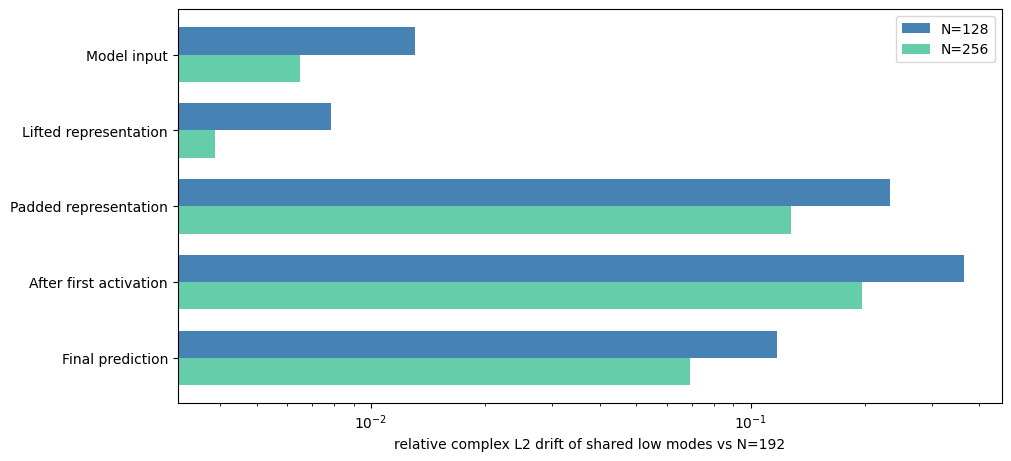
\includegraphics[width=0.9\textwidth]{figures/fno_internal_drift.png}
    \caption{Internal retained-mode drift of FNO k16 relative to the \(N=192\) forward pass. The inputs are spectrally resampled from the \(N=192\) fields. Drift is shown for selected stages of the model, with the largest increase occurring after spatial padding.}
    \label{fig:fno_internal_drift}
\end{figure}

Together, the FNO diagnostics give the following interpretation:
\begin{itemize}
    \item The loss increase at transfer resolutions is not explained simply by high-frequency target content outside the FNO cutoff, since most of the spectral error lies in the retained modes.
    \item Matching the retained input and target modes by spectral resampling does not recover the training-resolution behavior, showing that the mismatch is grid-dependent and introduced during the model forward pass.
    \item The largest layerwise increase in retained-mode drift occurs after spatial padding, identifying fixed-cell padding as the main source of resolution-dependent internal drift in the tested FNO.
\end{itemize}






\subsubsection{CNO high-resolution diagnostics}
\label{sec:cno_diagnostics}

The Navier--Stokes resolution-transfer results show that CNO\_standard and CNO\_no\_UND behave similarly over most of the evaluated range, but CNO\_no\_UND gives slightly lower loss at resolutions above the training resolution. This differs from the Darcy flow results, where CNO\_standard performs better at all evaluated resolutions. Since the only architectural difference between the two CNO variants is the upsample--nonlinearity--downsample block, additional diagnostics were performed to investigate this high-resolution Navier--Stokes behavior.

First, the filtering effect of the UND operation was measured directly. Individual Fourier modes were passed through the upsample--downsample part of the UND block, and the amplitude of the same mode after filtering was compared with its original amplitude. Figure~\ref{fig:cno_und_gain} shows the resulting same-mode gain \(G(k_x,k_y)\) at internal resolution \(N=192\). Values close to one indicate that the filter barely attenuates the mode, while lower values indicate stronger attenuation.

At the finest internal resolution, the UND operation is nearly identity on the lowest modes. In particular, the region where \(G(k_x,k_y)\approx1\) contains the modes used to generate the Navier--Stokes initial conditions. The gain then decreases smoothly toward higher wavenumbers, showing that the UND filter acts as a gradual low-pass operation rather than a sharp spectral cutoff.

The gain pattern should be interpreted relative to the bandwidth of the grid on which the UND operation is applied. At \(N=192\), the plotted quadrant extends to the Nyquist mode \(96\); if the spatial resolution is halved to \(N=96\), the same pattern extends only to mode \(48\). Thus, as the CNO encoder downsamples the feature maps, the same physical spatial variation occupies a larger fraction of the available bandwidth and can be more strongly affected by UND filtering in deeper layers.

\begin{figure}
    \centering
    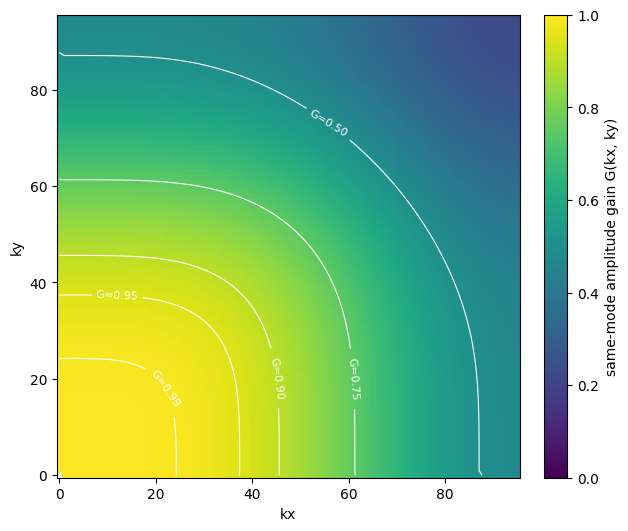
\includegraphics[width=0.85\textwidth]{figures/cno_und_gain.png}
    \caption{\label{fig:cno_und_gain}
    Same-mode amplitude gain \(G(k_x,k_y)\) of the standard UND upsample--downsample filtering operation at internal resolution \(N=192\). Values near one indicate that the filter has little effect on that mode, while lower values indicate stronger attenuation. The response is nearly identity for low modes and decreases smoothly toward higher wavenumbers.}
\end{figure}

Second, the prediction error of CNO\_standard and CNO\_no\_UND was decomposed by Fourier band at \(N=256\). Because CNO predictions are produced on the fixed internal grid before being resampled to the requested evaluation resolution, a comparison performed only after interpolation to \(N=256\) could mix model error with interpolation effects. To avoid this, the raw \(192\times192\) CNO outputs were compared with the \(N=256\) target projected to the same \(192\times192\) grid. This measures the quality of the native internal output representation before the final interpolation step.

On this raw output grid, CNO\_no\_UND obtains lower MSE than CNO\_standard:
\[
\mathrm{MSE}_{\mathrm{standard}} = 1.02\times 10^{-4},
\qquad
\mathrm{MSE}_{\mathrm{no\_UND}} = 8.54\times 10^{-5}.
\]
Figure~\ref{fig:cno_band_error_raw} shows the ratio between the bandwise spectral errors of the two models. For each Fourier band \(B\), the plotted value is
\[
\frac{E_B^{\mathrm{no\_UND}}}{E_B^{\mathrm{standard}}},
\qquad
E_B=\sum_{k\in B}|\hat u_{\mathrm{pred}}(k)-\hat u_{\mathrm{target}}(k)|^2,
\]
averaged over the test samples. Values below one therefore indicate bands where CNO\_no\_UND has lower error, while values above one indicate bands where CNO\_standard has lower error.

\begin{figure}
    \centering
    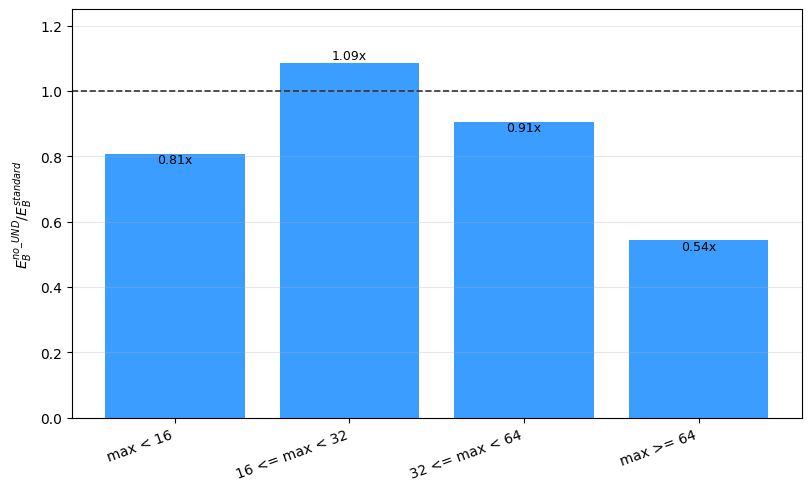
\includegraphics[width=0.8\textwidth]{figures/cno_band_error_raw_grid.png}
    \caption{\label{fig:cno_band_error_raw}
Ratio of box-band spectral error for CNO\_no\_UND relative to CNO\_standard on the raw \(192\times192\) output grid for inputs evaluated at \(N=256\). The \(N=256\) target is projected to the same \(192\times192\) grid before comparison. Here \(max\) is used as shorthand for \(\max(|k_x|,|k_y|)\), so the first band, \(max<16\), contains the modes used to generate the Navier--Stokes initial conditions. For each band \(B\), the plotted value is \(\frac{E_B^{\mathrm{no\_UND}}}{E_B^{\mathrm{standard}}}\), where \(E_B\) is the summed squared Fourier-coefficient error in that band, averaged over the test samples. The dashed line marks equal error. Values below one mean that CNO\_no\_UND has lower error; for example, \(0.81\times\) means that CNO\_no\_UND has \(81\%\) of the CNO\_standard error in that band, corresponding to a \(19\%\) reduction.}
\end{figure}

CNO\_no\_UND has lower error in the lowest band, where \(max<16\), with approximately \(81\%\) of the CNO\_standard error. It is slightly worse in the adjacent band, where \(16\leq max<32\), with approximately \(1.09\) times the CNO\_standard error, and has lower error again in the two higher bands. Since the comparison is performed on the raw \(192\times192\) output grid, this difference is already present before the final interpolation to \(N=256\).

Finally, spatial error maps were computed over the full Navier--Stokes test set at \(N=256\). Figure~\ref{fig:cno_spatial_error_maps} shows the mean squared-error maps for both CNO variants and their difference. Both models exhibit elevated error near the domain boundaries, indicating that these regions are difficult for both architectures. The difference map shows mixed behavior near the boundaries, with regions where CNO\_no\_UND improves and regions where it worsens. In the interior, the difference is smaller and more diffuse, indicating that the improvement is not localized to a single spatial structure.

\begin{figure}
    \centering
    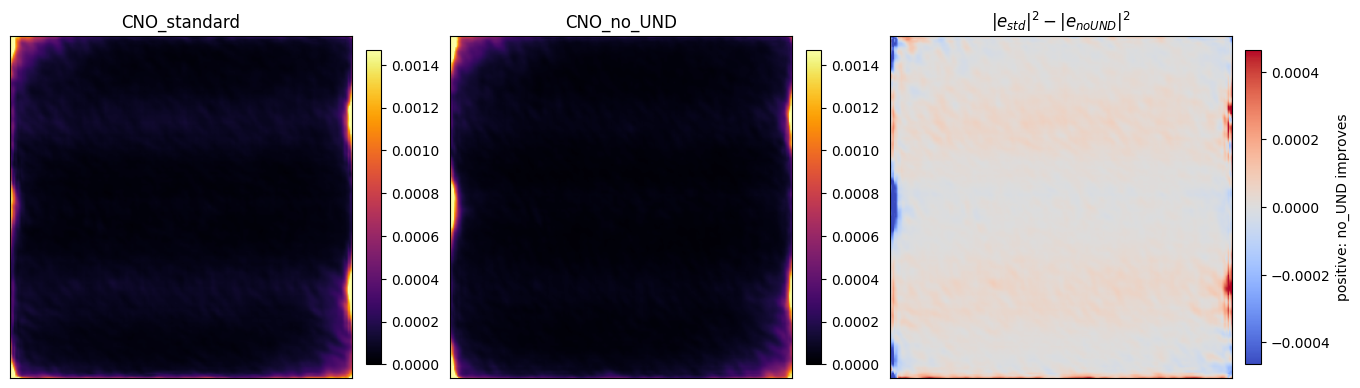
\includegraphics[width=0.95\textwidth]{figures/cno_spatial_error_maps.png}
    \caption{\label{fig:cno_spatial_error_maps}
    Mean spatial squared-error maps over the full Navier--Stokes test set at \(N=256\). The first two panels show the mean squared error for CNO\_standard and CNO\_no\_UND. The third panel shows the difference \(|e_{\mathrm{standard}}|^2-|e_{\mathrm{no\_UND}}|^2\), where positive values indicate regions where CNO\_no\_UND has lower error.}
\end{figure}

Together, the CNO diagnostics give the following interpretation:
\begin{itemize}
    \item The UND upsample--downsample operation acts as a gradual low-pass filter. At the finest internal resolution it barely attenuates the lowest Navier--Stokes modes, but the same filtering pattern becomes more restrictive at coarser internal resolutions where the available bandwidth is smaller.
    \item The high-resolution advantage of CNO\_no\_UND is already present on the raw \(192\times192\) output grid, so it is not primarily caused by the final interpolation to \(N=256\).
    \item The improvement is not only a high-frequency effect. CNO\_no\_UND has its largest practically important reduction in the lowest box band, indicating that removing UND changes the learned representation more broadly.
    \item The spatial error maps do not identify a single localized structure responsible for the improvement. The difference is distributed across the field, with mixed behavior near the boundaries.
\end{itemize}





\section{Discussion}

\subsection{FNO}\label{sec:fno_discussion}

The FNO variants show the weakest discretization robustness of the models tested on both datasets. This is most clearly visible in Figures~\ref{fig:loss_vs_resolution_navier_stokes} and~\ref{fig:loss_vs_resolution_darcy_flow}, where both FNO models show stronger dependence on evaluation resolution than the corresponding CNO models. The effect is particularly pronounced for FNO\_k16 on the Navier--Stokes dataset; FNO\_k16 achieves the lowest loss at the training resolution, but also has the largest value of \(D\) by a large margin. This shows that strong performance at the training resolution does not by itself imply robustness under resolution transfer.

The diagnostic experiments in Section~\ref{sec:fno_diagnostics} indicate that the behavior under resolution transfer is not primarily caused by the FNO simply discarding high-frequency target information. In Figure~\ref{fig:fno_error_bands}, the prediction error at the transfer resolutions is concentrated mainly in the modes explicitly retained by the FNO. At \(N=128\) and \(N=256\), the retained modes account for approximately \(93.3\%\) and \(95.1\%\) of the total spectral error, respectively. If the main issue were only that the target contained unresolved modes outside the spectral cutoff, the dominant error would instead be expected outside the retained band. The observed error distribution therefore points to a failure in the modes that the model is designed to represent directly. 

The spectral-resampling experiment in Table~\ref{tab:fno_spectral_resampling} further separates changes in the represented data from changes in model execution. With bicubic interpolation, the retained input and target modes differ from the \(N=192\) representation, especially at \(N=128\). However, when the \(N=128\) and \(N=256\) fields are constructed by spectral resampling from the \(N=192\) fields, the retained input and target drift is reduced to numerical precision. Despite this, the prediction drift remains large; approximately \(1.17\times10^{-1}\) at \(N=128\) and \(6.93\times10^{-2}\) at \(N=256\). This shows that the poor resolution transfer behavior is not explained simply by the retained Fourier coefficients of the input and target changing across spatial resolutions. Even when these retained coefficients are matched to numerical precision, the FNO still produces a substantially different prediction away from the training resolution. The remaining mismatch must therefore be introduced during the FNO forward pass itself.


The layerwise diagnostic in Figure~\ref{fig:fno_internal_drift} identifies where this resolution dependence enters the model. The model input already contains a small amount of drift relative to the \(N=192\) forward pass. The lifted representation remains at the same order of magnitude, indicating that the lifting layer does not substantially amplify this mismatch.

A much larger increase occurs after the spatial padding operation. For \(N=128\), the retained-mode drift increases from \(7.83\times10^{-3}\) in the lifted representation to \(2.33\times10^{-1}\) after padding. For \(N=256\), it increases from \(3.89\times10^{-3}\) to \(1.28\times10^{-1}\). The drift increases further after the first activation and remains elevated through the final prediction. This shows that the representations are still relatively close before padding, but diverge substantially once the padded representation is formed.

This points to fixed-cell spatial padding as the main implementation-level source of resolution dependence in the tested FNO. Because the FNO uses FFTs, the field passed to each spectral layer is implicitly treated as periodic. For non-periodic data, this creates an artificial discontinuity at the boundary of the periodic extension. Such discontinuities require many Fourier modes to represent and, after spectral truncation, can lead to ringing artifacts near the boundary.

To reduce this effect, the implementation applies zero padding in physical space before the Fourier layers. The Fourier operations are then applied on the enlarged padded domain, but only the original physical region is kept afterward. The padded region therefore acts as a buffer where boundary artifacts from the periodic extension can be absorbed without being directly penalized in the final loss. Equivalently, the model is not forced to make the two opposite edges of the physical domain match each other as they would in a strictly periodic representation.

However, the padding width in the original FNO implementation is specified as a fixed number of grid cells. If \(p\) cells are added to a grid of size \(N\), the physical width of the padded region scales like \(p/N\). Thus, the same padding value corresponds to different physical extensions at \(N=128\), \(N=192\), and \(N=256\). The Fourier transform inside the model is therefore applied to a resolution-dependent padded field rather than to the same physical field represented at different resolutions.

The consequence is that the Fourier transform inside the model is not applied to the same physical field represented at different resolutions. It is applied to different padded extensions of that field. Even if the unpadded input spectrum is held fixed, as in the spectral-resampling experiment, the object passed to the Fourier layers changes once padding is applied. This explains why the prediction still drifts when the retained input and target modes are matched to numerical precision. The learned spectral weights are being applied to internal representations that are no longer resolution-consistent.

This mechanism also explains why the FNO degrades both below and above the training resolution. In both cases, the physical width of the padded region differs from the one used during training. The degradation is stronger below the training resolution, which is likely compounded by the fact that coarser grids are more vulnerable to interpolation error, under-resolution, and possible aliasing. This is reflected in Table~\ref{tab:fno_spectral_resampling}, where bicubic interpolation produces a larger retained-mode input drift at \(N=128\) than at \(N=256\). These effects may contribute to the asymmetry of the loss curve, but they do not explain the main failure by themselves, since spectral resampling removes the input and target drift while the prediction drift remains large.

The particularly sharp minimum of FNO\_k16 on the Navier--Stokes dataset can therefore be understood as a combination of strong training-resolution accuracy and sensitivity to the exact discretization used during training. As described in Appendix~\ref{navier-details}, the initial vorticity fields are generated spectrally using modes with \(0<k_x,k_y<16\) in the positive quadrant, together with the corresponding conjugate modes needed to obtain real-valued fields. An FNO retaining 16 modes is therefore able to represent all Fourier modes present in the initial condition within its spectral layers. This does not mean that the final vorticity field is bandlimited to 16 modes, since the Navier--Stokes dynamics are nonlinear and generate additional higher-frequency content during time evolution. However, it does make FNO\_k16 especially well matched to the input representation at the training resolution, allowing it to achieve a very low loss at \(N=192\). When the same model is evaluated at another resolution, the internal representation changes through the coordinate grid and fixed-cell padding, producing the sharp increase in loss away from the training resolution observed in Figure~\ref{fig:loss_vs_resolution_navier_stokes}.

The comparison between FNO\_k8 and FNO\_k16 should be interpreted in this context. FNO\_k16 can treat all Fourier modes present in the initial Navier--Stokes condition explicitly through its spectral layers. It can therefore rely heavily on the retained Fourier coefficients when learning the mapping at the training resolution. This helps explain its very low loss at \(N=192\), but also makes the model sensitive when those internal coefficients change under resolution transfer. FNO\_k8, by contrast, retains only part of the Fourier content present in the initial condition. A larger fraction of the mapping must therefore be represented indirectly through the pointwise channel mixing and nonlinearities. This makes FNO\_k8 less accurate, but also less dependent on the full retained spectral representation being exactly the same as during training. As a result, FNO\_k8 shows a much lower value of \(D\), while FNO\_k16 gives better absolute accuracy but is more strongly tied to the training-resolution computation.

On the Darcy flow dataset, the same qualitative behavior appears but is less extreme. The Darcy input fields are not constructed to match the FNO\_k16 spectral cutoff in the same direct way as the generated Navier--Stokes initial conditions. As a result, FNO\_k16 does not receive the same artificial advantage of being able to represent essentially all input variation through its retained spectral modes. The difference between FNO\_k8 and FNO\_k16 is therefore less pronounced. Nevertheless, FNO\_k16 still benefits from the additional retained modes near the training resolution, while FNO\_k8 can be more stable at sufficiently low resolutions because it relies less strongly on a larger set of resolution-dependent spectral coefficients. This is consistent with the broader trade-off observed for the FNO models: retaining more modes improves accuracy when the evaluation representation matches training, but can increase sensitivity when the model is executed on a different grid.

The use of fixed-cell padding is not unreasonable in itself. It is simple to implement, keeps tensor sizes predictable, and is harmless when training and evaluation are performed at a single fixed resolution. It becomes problematic when the trained FNO is evaluated at resolutions different from the one used during training. In that setting, a fixed number of padded cells corresponds to a different physical padding width, so the model no longer applies the Fourier layers to the same padded representation of the physical domain. This reintroduces discretization dependence into an architecture that is otherwise often described as resolution-flexible.





\subsection{CNO}
\label{sec:cno_discussion}

In contrast to the FNO, the CNO variants show substantially stronger consistency across evaluation resolutions on both datasets. This is visible in Figures~\ref{fig:loss_vs_resolution_navier_stokes} and~\ref{fig:loss_vs_resolution_darcy_flow}, where the CNO loss curves are much flatter than those of FNO\_k16. The corresponding values of \(D\) are also substantially smaller, especially on the Darcy flow dataset. This supports the central design idea of the CNO: before the main encoder--decoder operator is applied, all inputs are mapped onto a fixed internal grid. The convolutional kernels, downsampling operations, and upsampling operations therefore act on the same internal discretization during training and evaluation.

The same design also introduces a limitation. Since the CNO always predicts through a fixed internal resolution, it cannot represent arbitrary additional information that becomes available at higher evaluation resolutions. When the evaluation resolution is increased beyond the internal grid, the prediction is still produced on the internal grid and then resampled to the requested resolution. The high-resolution loss therefore measures not only the model error, but also the mismatch between the true high-resolution target and what can be represented through the fixed internal grid. This is why the CNO loss increases gradually at higher resolutions rather than remaining perfectly constant, and the rate at which it increases depends on how well the internal grid can represent the relevant solution structure at the higher resolution.

This interpretation is clearest on the Darcy flow dataset. The Darcy solution fields are comparatively smooth, and the relevant solution structure is well represented at the internal resolution. As a result, both CNO variants show very small values of \(D\), and the standard CNO performs best across all evaluated resolutions. In this setting, the fixed internal grid removes most resolution dependence without discarding much physically relevant information. The UND block is also beneficial here, since the additional anti-aliasing constraint improves representation consistency without noticeably limiting the model.

The Navier--Stokes results require a closer look at the role of the UND block. CNO\_standard and CNO\_no\_UND behave similarly across most resolutions, but CNO\_no\_UND slightly outperforms the standard CNO above the training resolution. Since the UND block is the only architectural difference between the two models, the diagnostics in Section~\ref{sec:cno_diagnostics} were used to examine how this block changes the model behavior.

To isolate the effect of the UND filter, individual Fourier modes were passed through only the upsampling and downsampling operations used in the UND block. Figure~\ref{fig:cno_und_gain} shows that the filter is close to identity for the lowest modes at the finest internal resolution, while its gain decreases smoothly toward higher wavenumbers. Thus, the UND block does not impose a sharp spectral cutoff, but it does introduce gradual frequency-dependent attenuation.

This gain map should be interpreted in the context of both the Navier--Stokes spectra and the multiscale CNO architecture. The initial conditions are generated using modes with \(|k_x|,|k_y|<16\), while the final states contain substantial energy up to roughly twice this range, as shown in Appendix~\ref{navier-details}. At the finest internal resolution, these modes lie in a region where the UND filter is close to identity, so the finest-scale UND block is unlikely to remove the dominant physical frequencies directly. However, the CNO applies UND blocks throughout the encoder--decoder. For the Navier--Stokes CNOs, the finest internal resolution is \(192\times192\), while the coarsest encoder resolution is \(24\times24\), reducing the Nyquist mode from \(96\) to \(12\). Physical structures represented by modes around \(k=16\) or \(k=32\) are therefore well inside the available bandwidth at the finest scale, but near or beyond it at the coarsest scale. The UND filter can consequently affect physically relevant feature content more strongly in deeper layers than the finest-resolution gain map alone suggests.

The output diagnostics rule out two simple explanations for the high-resolution CNO\_no\_UND advantage. First, Figure~\ref{fig:cno_band_error_raw} shows that the difference is already present on the raw \(192\times192\) output grid, before the final interpolation to \(N=256\). The improvement is therefore not primarily an interpolation artifact. Second, the advantage is not simply a high-frequency preservation effect. CNO\_no\_UND has lower error in the lowest band, \(max<16\), with approximately \(81\%\) of the CNO\_standard error, while it is slightly worse in the adjacent band \(16\leq max<32\). The improvement is therefore distributed across the representation rather than isolated to the highest modes.

A plausible remaining explanation is that removing UND gives the model access to additional aliased components generated by nonlinear activations. In the standard CNO, the activation is applied on an upsampled grid and then low-pass filtered before returning to the original resolution, reducing aliasing and enforcing representation consistency \cite{bartolucci-discretization-invariance}. Without this step, frequencies generated above the grid bandwidth can fold back into represented modes and be passed to later layers. These aliased components are not guaranteed to correspond to meaningful continuous features, but they can still act as additional discrete degrees of freedom for reducing finite-resolution loss. Since aliasing maps unresolved high-frequency content into lower represented modes, this mechanism can also affect the low-mode error observed in Figure~\ref{fig:cno_band_error_raw}.

This interpretation is consistent with the fact that the advantage appears only above the training resolution, although it is not proven conclusively by the diagnostics. At higher evaluation resolutions, the fixed internal representation becomes a bottleneck: the model must produce a \(192\times192\) field whose resampled version approximates a more finely resolved target. For the Navier--Stokes case, where nonlinear dynamics transfer energy across spatial scales and the final state contains broader spectral content than the initial condition, the additional aliased components available to CNO\_no\_UND may help form a native \(192\times192\) representation that better matches the projected high-resolution target. At the training resolution and below, the benefit of these components is less clear, while the anti-aliasing and representation consistency of the standard CNO remain advantageous.

The spatial error maps in Figure~\ref{fig:cno_spatial_error_maps} suggest that the difference is not a purely local effect. Both models have elevated error near the boundaries, which is expected for a convolutional encoder--decoder because convolutional stencils are incomplete at the edge of the domain and are evaluated using padding. Repeated downsampling and upsampling can then propagate these boundary effects across scales. The difference map shows mixed behavior near the boundaries rather than a single region where CNO\_no\_UND consistently improves. The improvement is therefore better understood as a change in the learned discrete representation as a whole, rather than as a correction of one specific spatial feature.

This should not be interpreted as evidence that the UND block is generally harmful. On the Darcy flow dataset, CNO\_standard performs better at all evaluated resolutions, and on Navier--Stokes it performs as well or better over most of the evaluated range. Indeed, the UND construction is central to the representation-consistency argument for the CNO as a neural operator \cite{bartolucci-discretization-invariance}. The result should instead be understood as an empirical trade-off. The standard CNO enforces stronger aliasing control and representation consistency, while CNO\_no\_UND allows aliasing generated by nonlinear activations to remain part of the finite-grid representation. For the high-resolution Navier--Stokes evaluations considered here, these additional discrete signals slightly improve MSE, but they do not make CNO\_no\_UND the more theoretically discretization-invariant model.

Overall, the CNO results show that fixed internal resampling is the dominant reason for the improved resolution robustness relative to the FNO. The role of UND is more nuanced. It improves representation consistency and is beneficial on the smoother Darcy benchmark, but in the high-resolution Navier--Stokes regime it can be slightly outperformed by the less constrained no\_UND variant. The diagnostics therefore support a view of CNO robustness as a balance between two effects: enforcing a stable internal discretization and controlling nonlinear aliasing without overly restricting the discrete representations useful for prediction.



\subsection{Improving the FNO}
\label{sec:improving_fno}

\begin{figure}
    \centering
    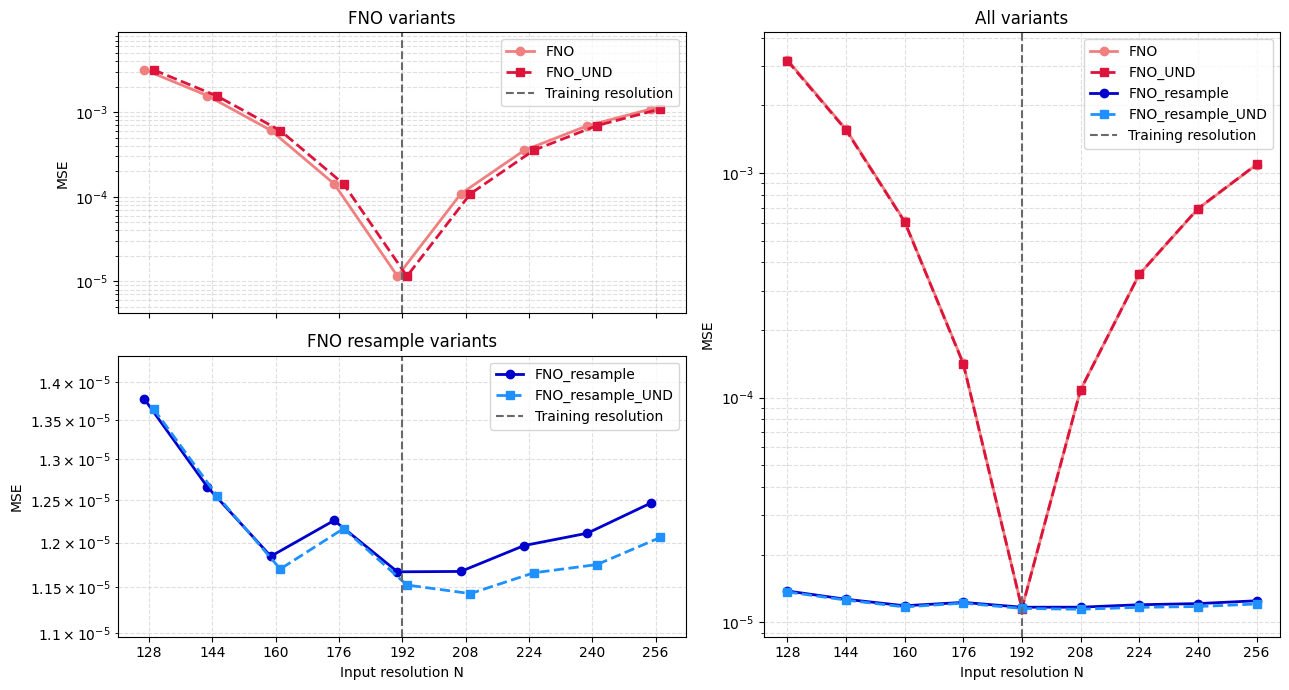
\includegraphics[width=0.8\textwidth]{figures/improving_fno.png}
    \caption{\label{fig:improving-fno} MSE loss as a function of evaluation resolution for four FNO variants trained on the Navier--Stokes dataset. The left panels separate the nearly overlapping curves for readability: the top panel compares the standard FNO and FNO\_UND, while the bottom panel compares FNO\_resample and FNO\_resample\_UND. A small horizontal offset is applied to the curves in these two panels only to make both models visible. The right panel shows all four variants on the same axes without offset. The vertical dashed lines mark the training resolution.
}
\end{figure}

The previous section identified resolution-dependent internal representations as the main source of poor resolution transfer in the standard FNO. In particular, the layerwise diagnostic in Figure~\ref{fig:fno_internal_drift} showed that the internal representation changes sharply after fixed-cell padding. This suggests that the FNO may benefit from the same fixed-grid strategy used in the CNO, where the main learned operator is applied on a consistent internal discretization rather than directly on the input grid.

To test this, two modifications inspired by the CNO were added to the FNO. The first is fixed-grid resampling, where all inputs are first resampled onto the training resolution before being passed through the FNO. The second is the UND block, which is designed to reduce aliasing introduced by nonlinear activations. These modifications were tested separately and in combination, giving four models: the standard FNO, FNO\_UND, FNO\_resample, and FNO\_resample\_UND. All four models retained 16 Fourier modes in each direction and were trained and evaluated on the Navier--Stokes dataset.

\begin{table}
    \centering
    \caption{\label{tab:d-values-navier-stokes-improved-fno} Values of \(D\) for the modified FNO models on the Navier--Stokes dataset. Lower values of \(D\) indicate more consistent loss across evaluation resolutions.}
    \begin{tabular}{lc}
        \hline
        Model & \(D\) \\
        \hline
        FNO & 3.4817 \\
        FNO\_UND & 3.4800 \\
        FNO\_resample & 0.0490 \\
        FNO\_resample\_UND & 0.0456 \\
        \hline
    \end{tabular}
\end{table}

The results are shown in Figure~\ref{fig:improving-fno}, with the corresponding values of \(D\) reported in Table~\ref{tab:d-values-navier-stokes-improved-fno}. Adding the UND block alone produces almost no change. The value of \(D\) changes from 3.4817 for the standard FNO to 3.4800 for FNO\_UND, indicating that nonlinear aliasing from the activation functions is not the dominant source of the observed resolution dependence.

In contrast, fixed-grid resampling produces a large improvement. FNO\_resample reduces \(D\) from 3.4817 to 0.0490, while FNO\_resample\_UND gives a similar value of 0.0456. This supports the interpretation developed in Section~\ref{sec:fno_discussion}: the main issue is not the Fourier basis alone, nor simply the finite number of retained modes, but the fact that the standard FNO executes its learned computation on the evaluation grid. When the evaluation resolution changes, the coordinate representation, padding operation, Fourier transforms, and spectral weights are applied to a different internal representation than the one seen during training.

Fixed-grid resampling avoids this by ensuring that the FNO layers are always applied at the same internal resolution. In particular, the fixed-cell padding is then applied after the input has been mapped to the training resolution, so the padded region has the same physical meaning during training and evaluation. This removes the dominant source of internal representation drift identified in Figure~\ref{fig:fno_internal_drift}.

The small additional improvement from combining resampling with the UND block suggests that aliasing from nonlinear activations may still contribute slightly once the dominant representation mismatch has been removed. However, the difference between FNO\_resample and FNO\_resample\_UND is minor compared with the improvement caused by fixed-grid resampling itself.

These results show that the poor discretization robustness of the standard FNO is strongly linked to the fixed-cell padding operation. When the model is evaluated directly at a different spatial resolution, the same number of padded cells corresponds to a different physical padding width than during training. Mapping all inputs to the training resolution before applying the FNO removes this padding mismatch, so the Fourier layers and padding operation act on the same internal representation during both training and inference.